\newpage

\paragraph{ }

\newpage


\section{Appendix}
\subsection{Neighborhood Attention (NA)}
\label{sec:na}
Neighborhood Attention (NA)\cite{NAdeliated} is a local attention pattern used for 2D images, in which each pixel attends to its nearest neighboring pixels. 
NA mask is very complicated (Figure \ref{fig:natten_masks} top left) due to the 1D expansion of a 2D embedding neighborhood and thereby makes NA challenging to compute. 
Various advanced expansion strategies have been proposed\cite{NAtiled, NAfaster} to improve its block sparsity, but it is challenging manually to implement these optimizations in a high-performance attention kernel. 
Instead, we showcase that with \textit{FlexAttention}, the Tiled NA and Morton curve NA could be implemented in less than 10 lines of PyTorch code to exploit the sparsity of NA (Figure \ref{fig:natten_masks}) and enjoy its performance benefits (Figure \ref{fig:evaluation:natten}). 








\begin{figure}[!h]
    \centering
    \begin{tabular}{@{}c@{}@{}c@{}}

    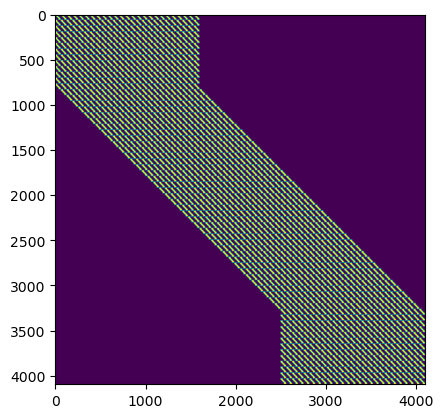
\includegraphics[width=0.37\linewidth]{graphs/Mask_NATTEN.png} & 
    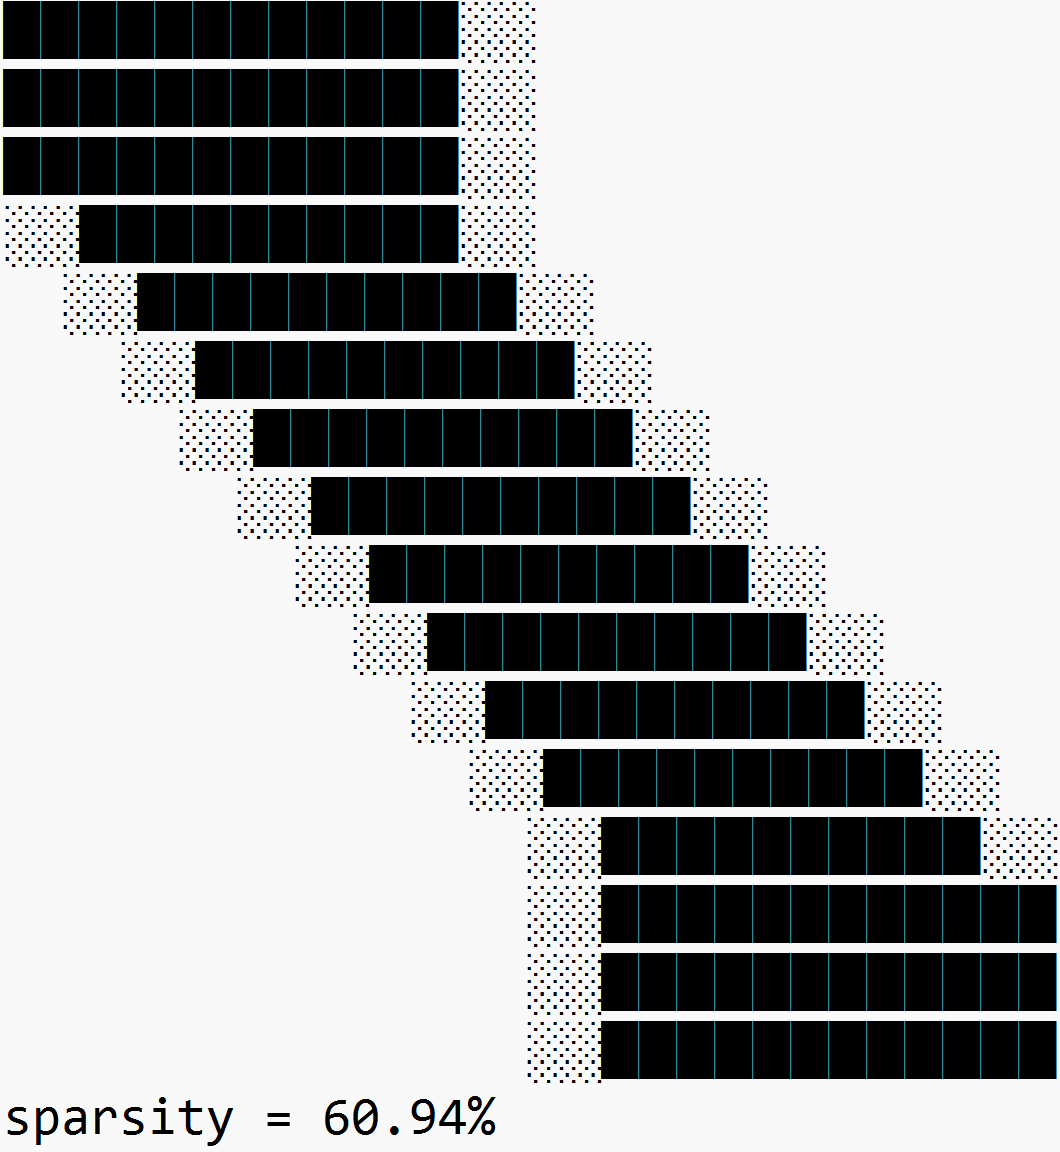
\includegraphics[width=0.3\linewidth]{graphs/BlockMask_NATTEN.png} \\
    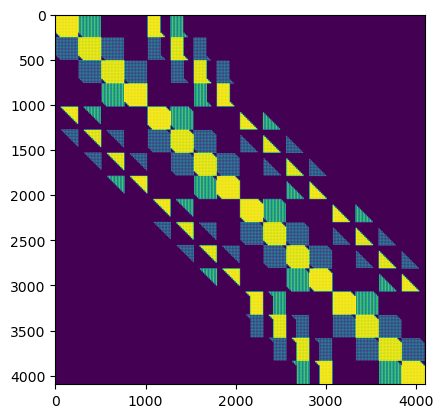
\includegraphics[width=0.37\linewidth]{graphs/Mask_tiled_NATTEN.png} & 
    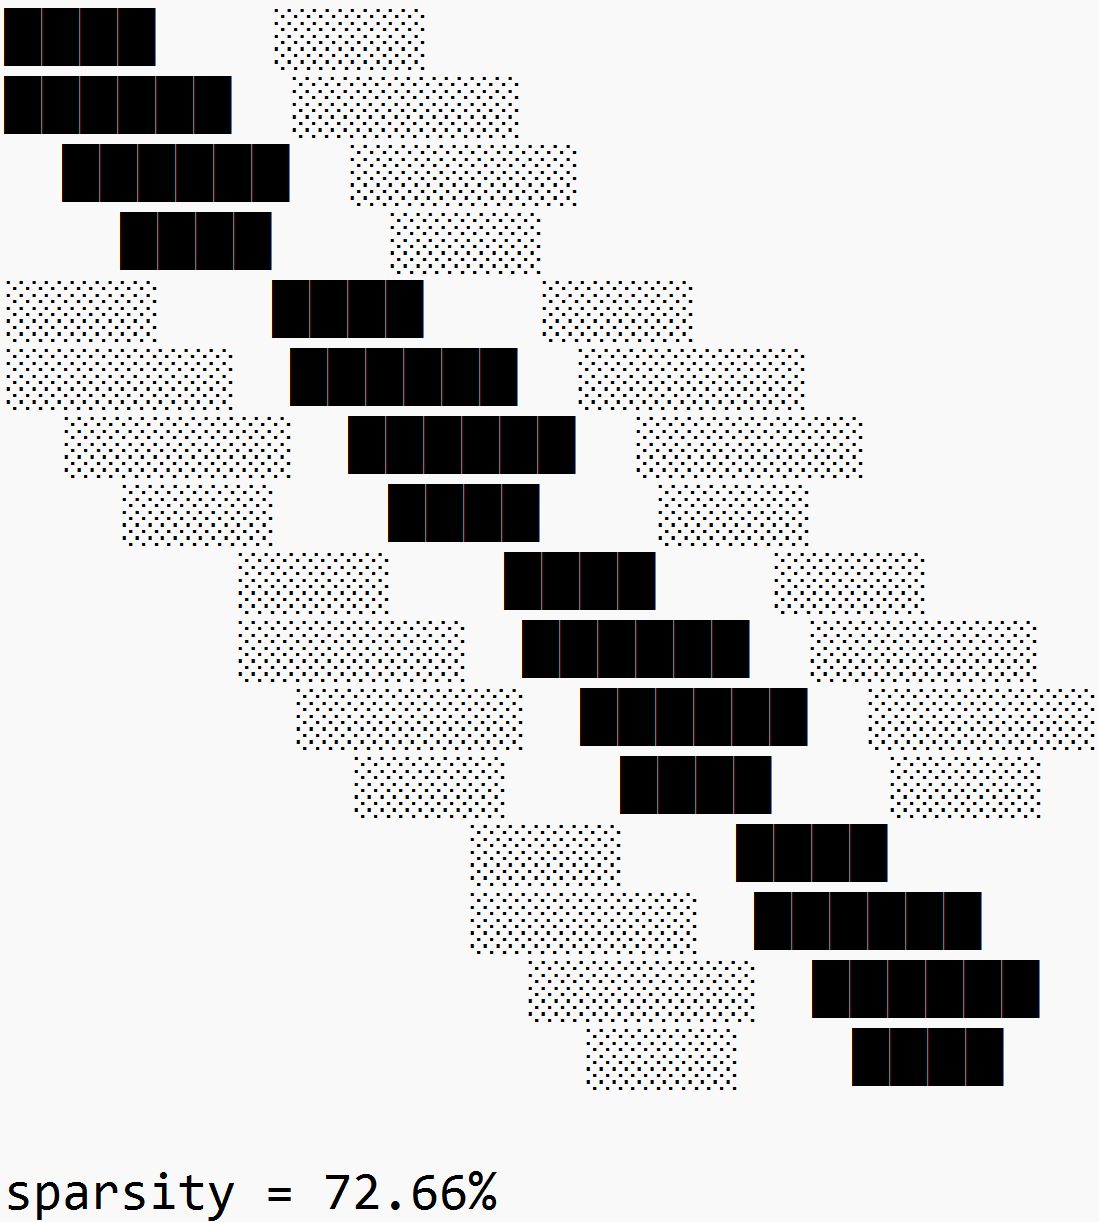
\includegraphics[width=0.3\linewidth]{graphs/BlockMask_tiled_NATTEN.png} \\
    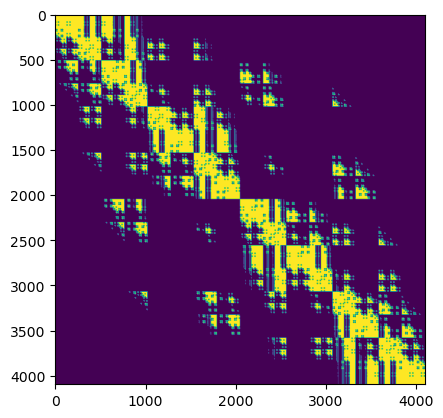
\includegraphics[width=0.37\linewidth]{graphs/Mask_morton_NATTEN.png} & 
    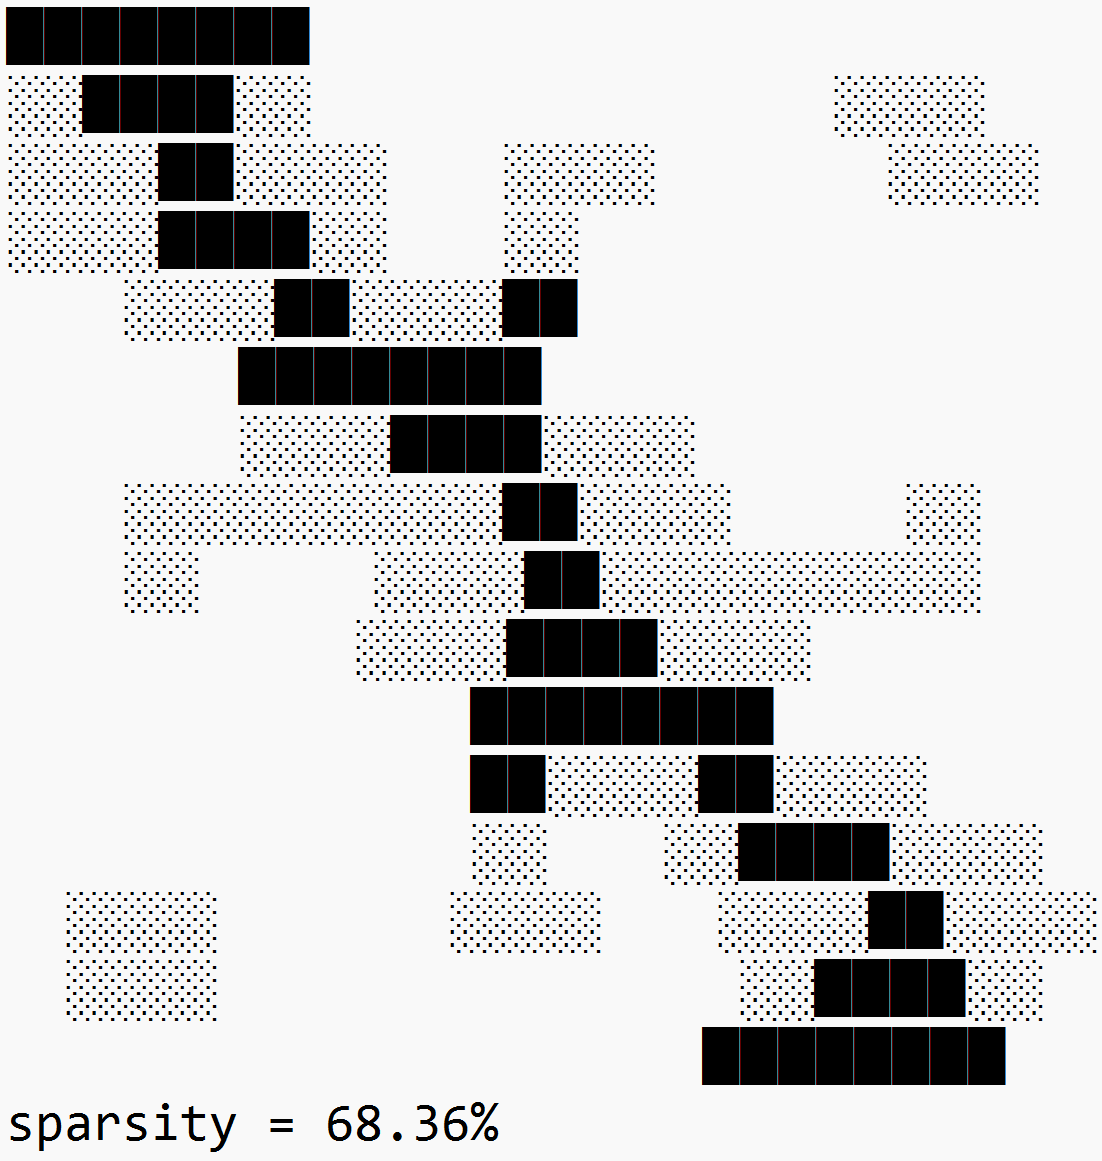
\includegraphics[width=0.3\linewidth]{graphs/BlockMask_NATTEN_Hilbert.png} \\
  \end{tabular}
    \caption{NA Itemized Mask and the Corresponding Block Mask. \textbf{Top: } Naive NATTEN Mask. \textbf{Middle: } 2D-Tiled NA Mask. \textbf{Bottom: } Morton Curve NA Mask.}
    \label{fig:natten_masks}
\end{figure}







% \subsection{Case Study: Neighborhood Attention}
\begin{figure}[!h]
    \centering
  \begin{subfigure}
         \centering
         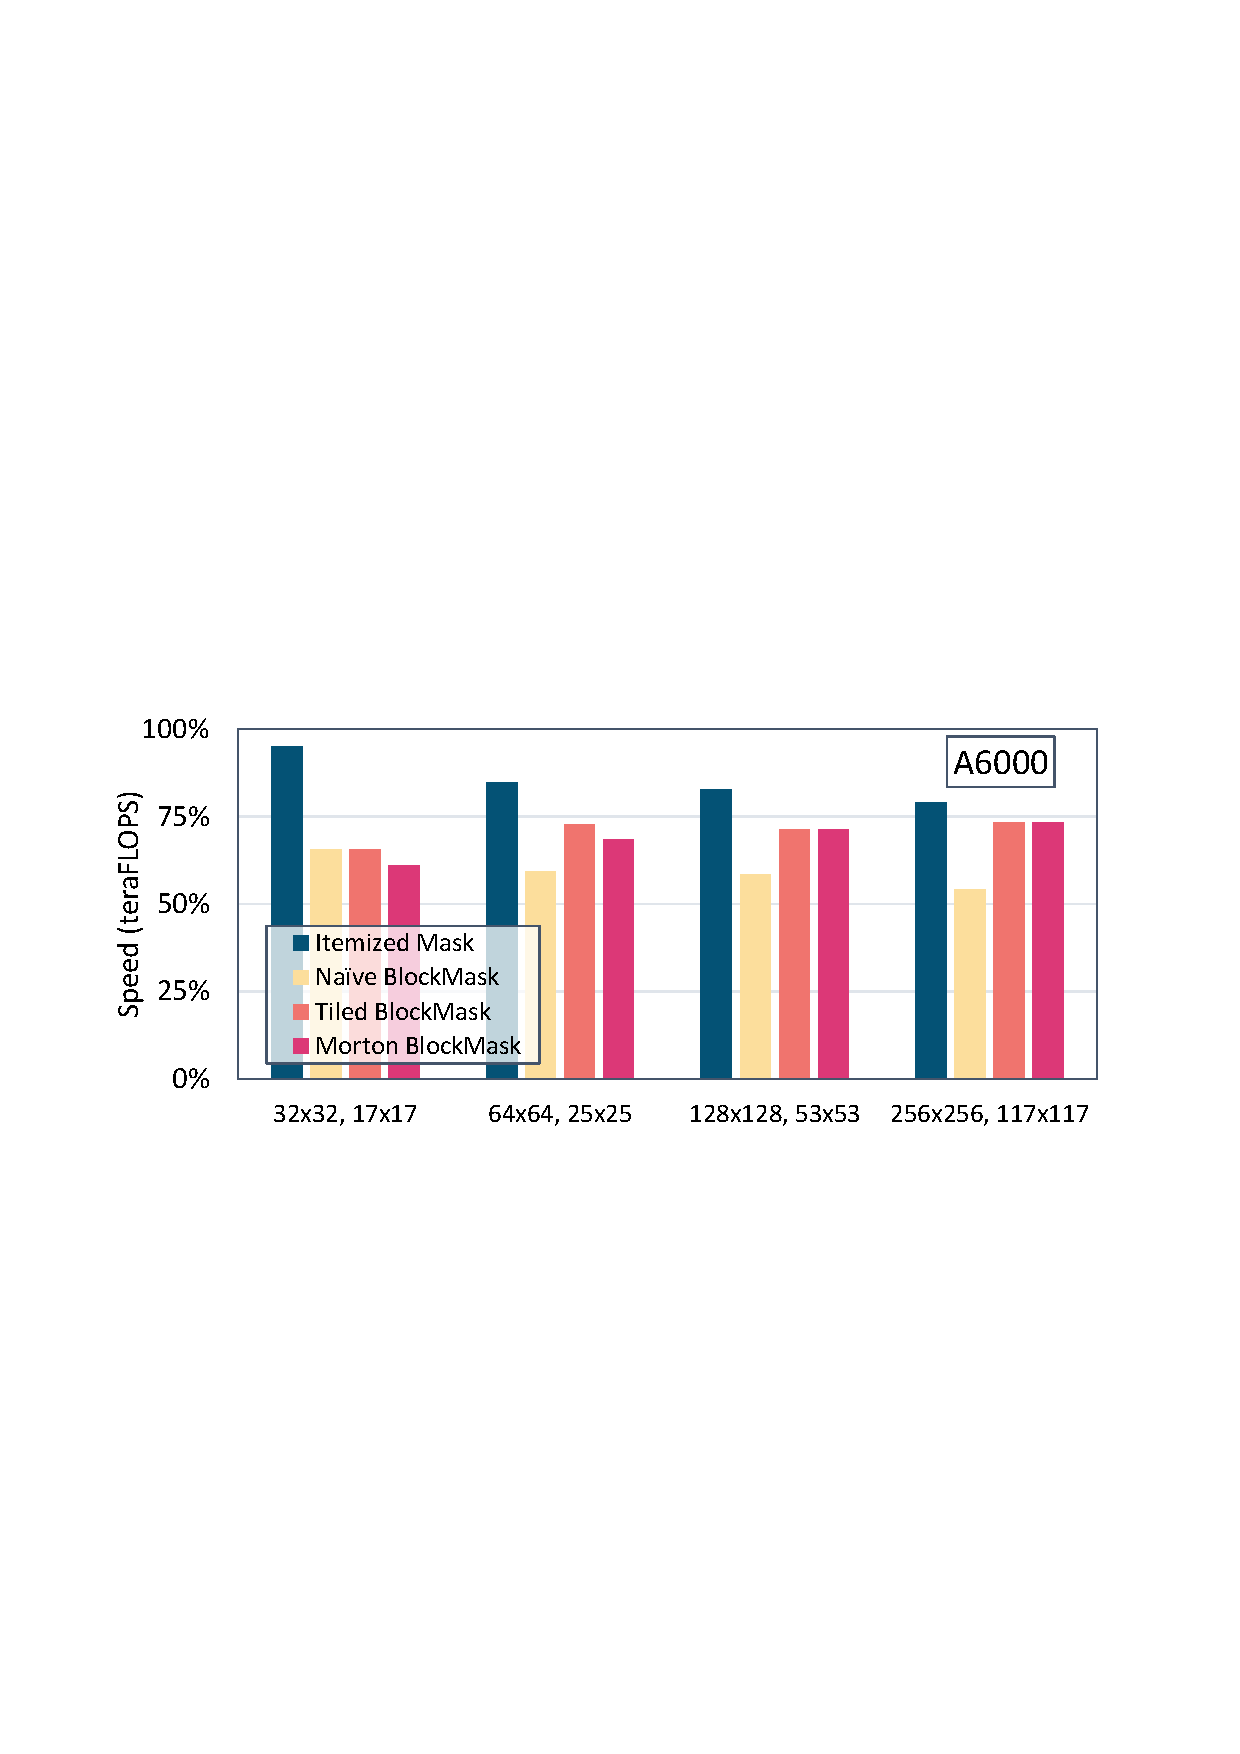
\includegraphics[width=\linewidth]{graphs/NATTEN_sparsity.pdf}
    \end{subfigure}
    % removed to save space
    %  \hfill
    %  \begin{subfigure}
    %      \centering
    %      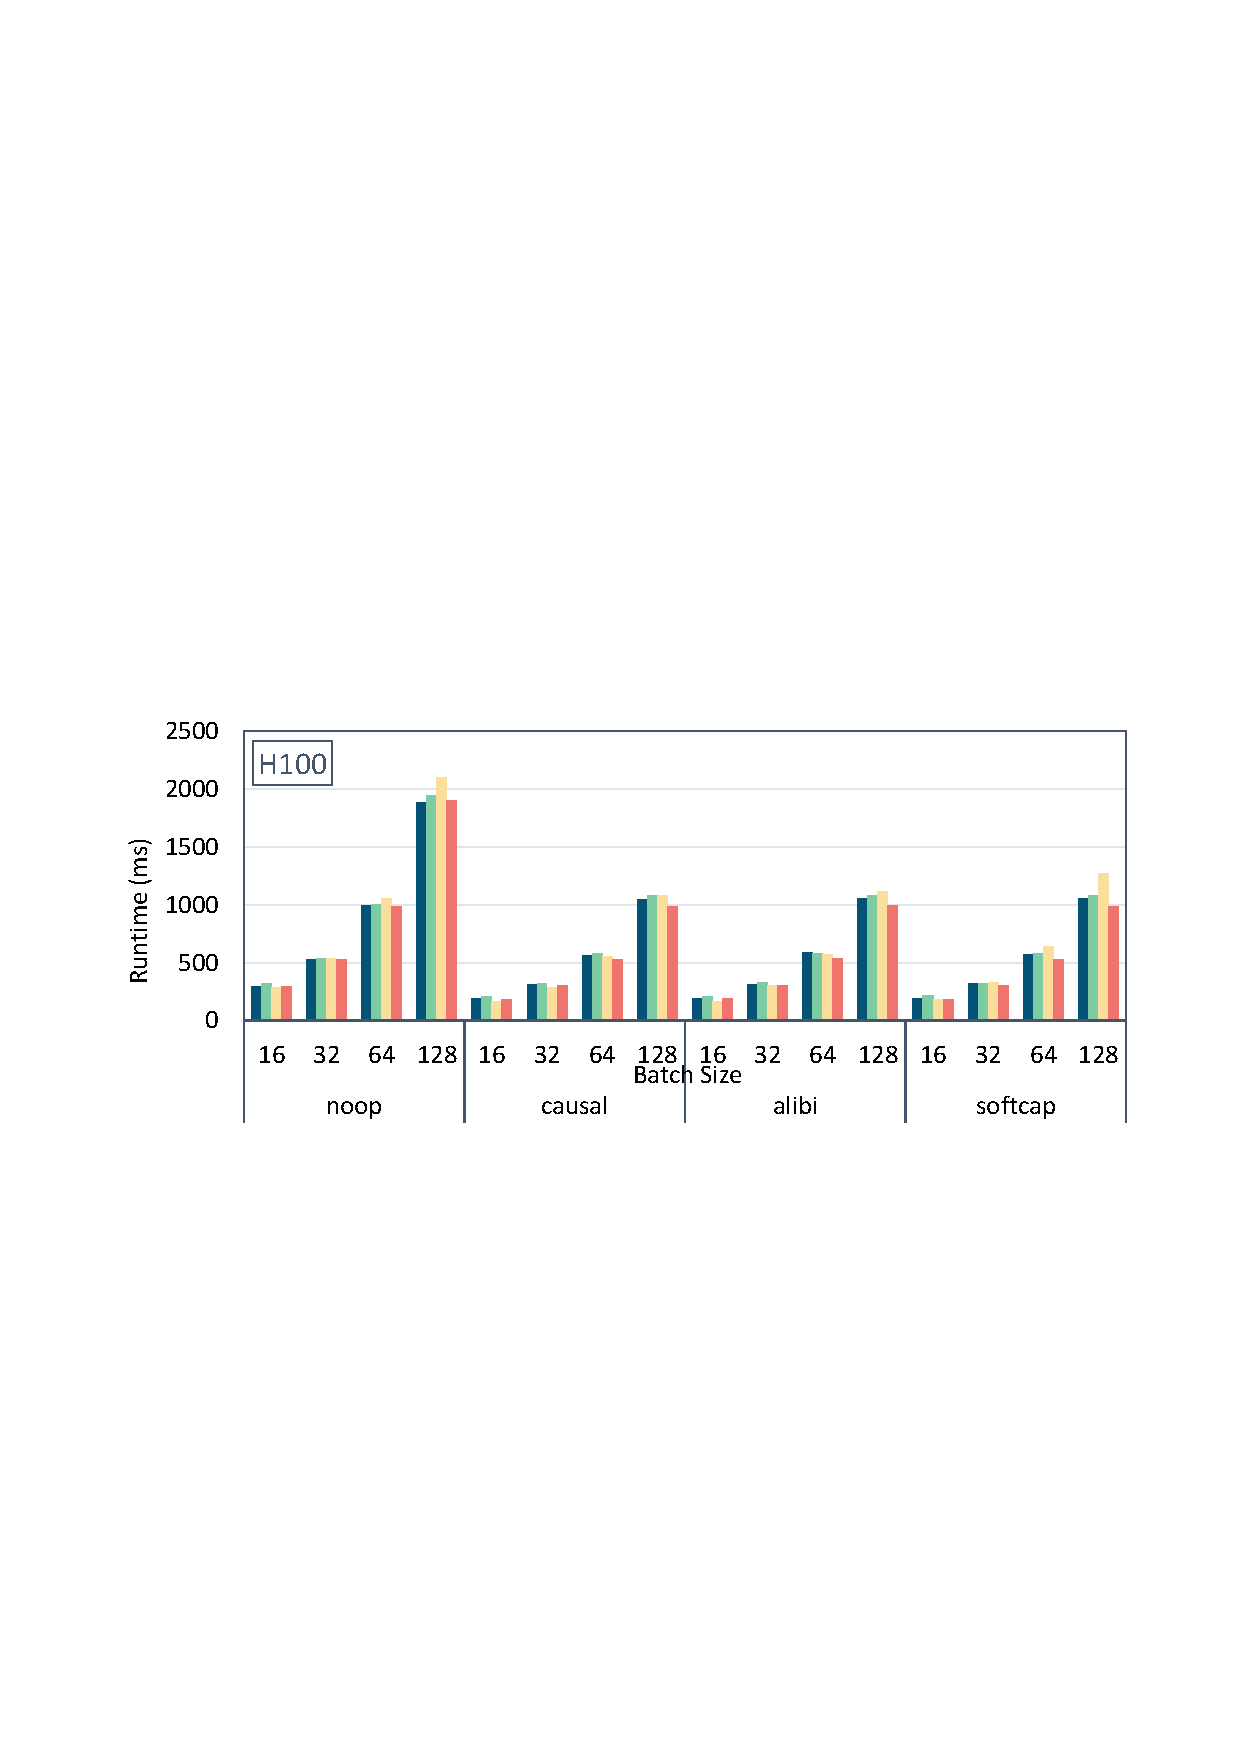
\includegraphics[width=\linewidth]{graphs/PagedBsz.pdf}
    % \end{subfigure}
    \hfill
    \begin{subfigure}
         \centering
         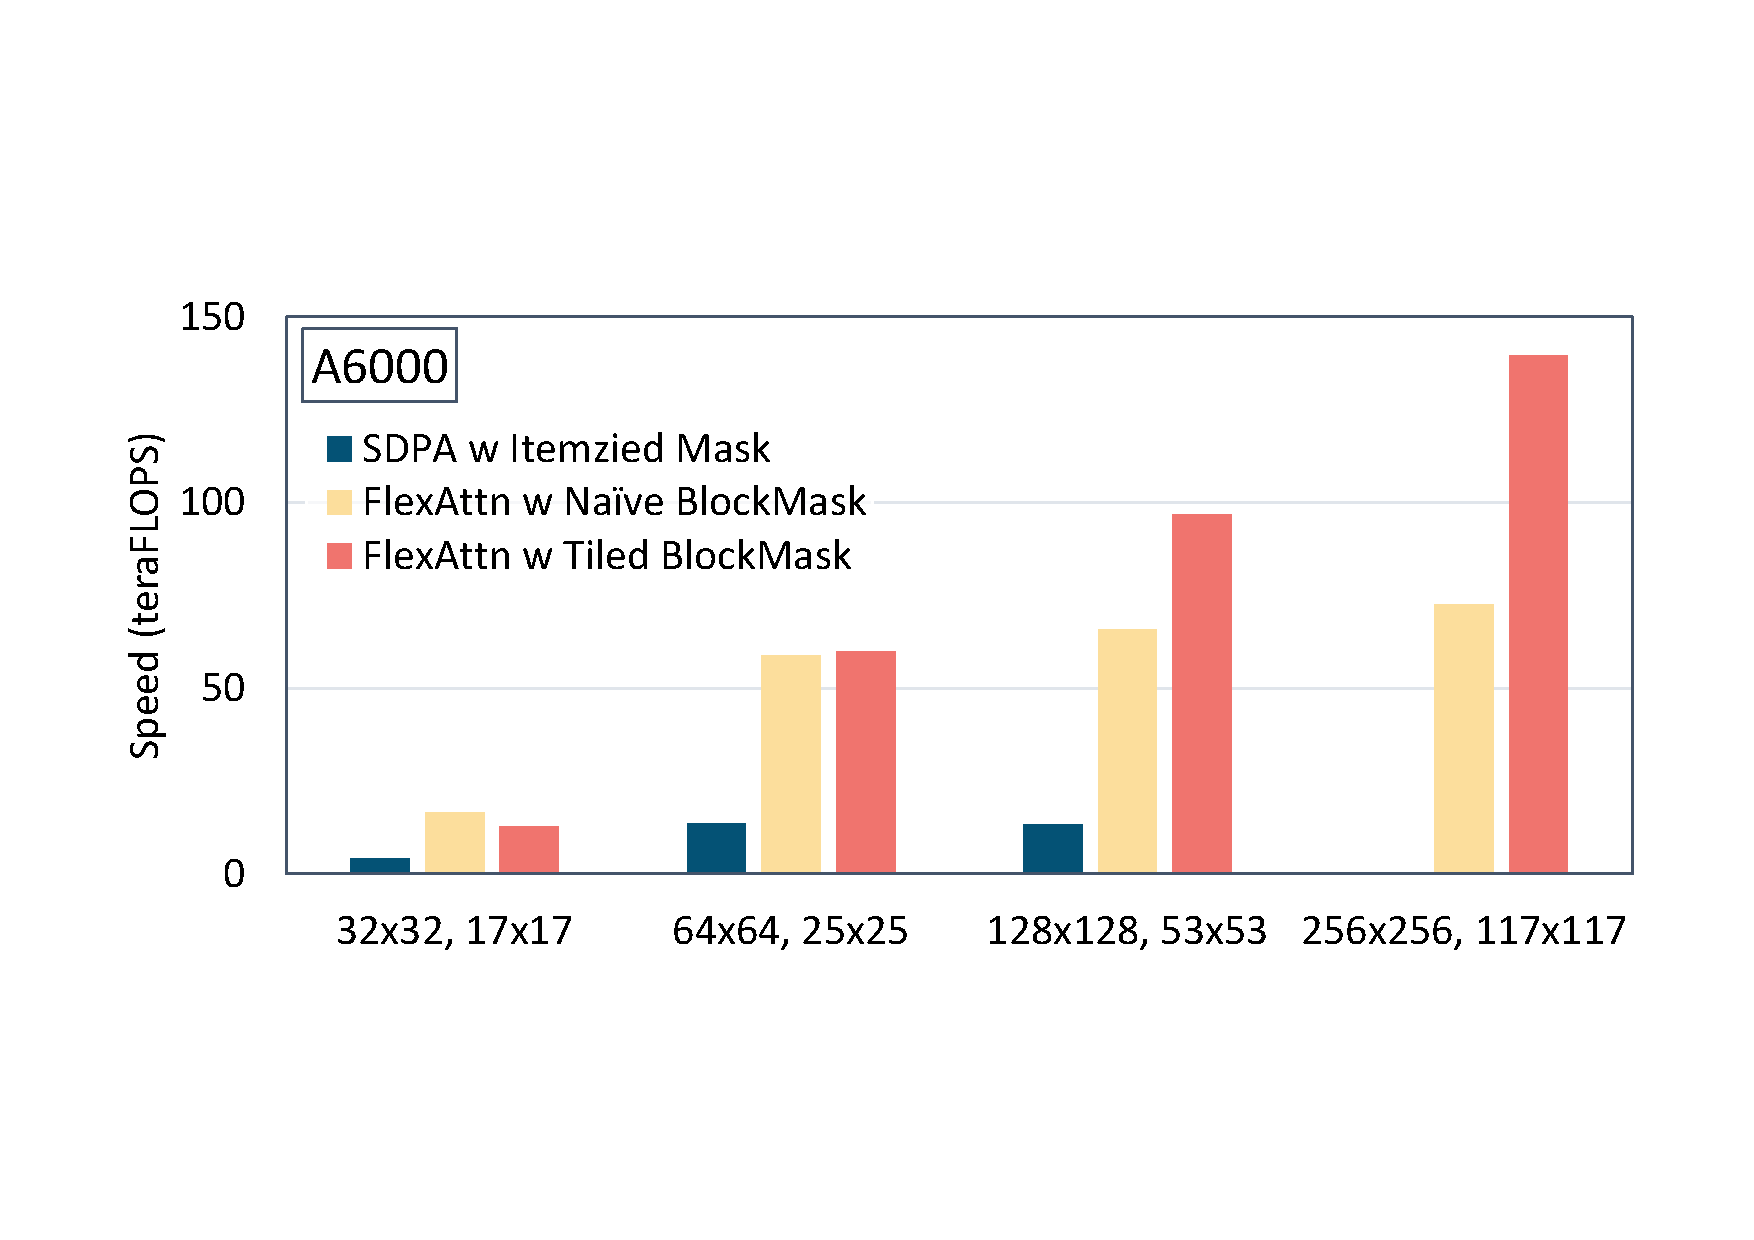
\includegraphics[width=\linewidth]{graphs/NATTEN_performance.pdf}
    \end{subfigure}
    \caption{Neighborhood Attention with Different Mapping w.r.t canvas size, kernel size. \textbf{Top:} Mask Sparsity. \textbf{Bottom:} Speed.}
    \label{fig:evaluation:natten}
\end{figure}